\documentclass[aspectratio=169]{beamer}

\usepackage{graphicx}
\usepackage{amsmath,amssymb,bm}
\usepackage{ragged2e}
\usepackage{tikz}
\usepackage{xcolor}
\usepackage{array}
\usepackage{booktabs}

\usetikzlibrary{arrows.meta,positioning,calc}
\graphicspath{{figures/}}

\definecolor{maroon1}{rgb}{0.478, 0, 0.235}
\definecolor{maroonDim}{RGB}{108,43,72}
\definecolor{blockTint}{RGB}{246,244,247}
\definecolor{lightgray}{rgb}{0.94,0.94,0.97}
\definecolor{lightgray2}{rgb}{0.5,0.5,0.5}
\definecolor{maccblue}{RGB}{28,74,117}
\definecolor{maccgreen}{RGB}{44,118,92}
\definecolor{maccred}{RGB}{156,58,52}
\definecolor{maccorange}{RGB}{216,100,42}

\usetheme{Copenhagen}
\usecolortheme[named=maroon1]{structure}

\setbeamerfont{caption}{size=\scriptsize}
\setbeamertemplate{navigation symbols}{}
\setbeamertemplate{blocks}[rounded][shadow=false]
\setbeamercolor{block body}{fg=black,bg=blockTint}
\setbeamercolor{block title}{fg=white,bg=maroonDim}

\newcommand{\FH}{F_H}
\newcommand{\FA}{F_A}
\newcommand{\FW}{F_W}
\newcommand{\FT}{F_T}
\newcommand{\FB}{F_B}
\newcommand{\Cbuf}{C_{\mathrm{buf}}}
\newcommand{\pH}{\mathrm{pH}}

\expandafter\def\expandafter\insertshorttitle\expandafter{%
\insertshorttitle\hfill%
\insertframenumber\,/\,\inserttotalframenumber}

\title[pH Supervisor Update]{pH Modeling Update}
\author[A. H. Hamedi]{A. H. Hamedi}
\date[June 2026]{June 24, 2026}

\begin{document}

%============================= Slide 1 ============================
\begin{frame}
\setbeamertemplate{blocks}[rounded][shadow=false]
\setbeamercolor{block body}{fg=black,bg=blockTint}
\frametitle{\large \textbf{HH is the baseline because water cancels from the ideal ratio}}
\scriptsize

\vspace{-0.18cm}
\begin{columns}[T,onlytextwidth]
\begin{column}{0.43\textwidth}
\begin{block}{Acetate-buffer model}
\vspace{-0.14cm}
\[
  C_{HA}=\frac{C_0\FH}{\FH+\FA+\FW},
  \qquad
  C_{A^-}=\frac{C_0\FA}{\FH+\FA+\FW}
\]
\vspace{-0.20cm}
\[
  \pH \approx pK_a+\log_{10}\frac{C_{A^-}}{C_{HA}}
  \approx pK_a+\log_{10}\frac{\FA}{\FH}
\]
\vspace{-0.16cm}
\end{block}

\vspace{0.04cm}
\begin{block}{Small interpretation}
\justifying
Water should not be forced to explain steady-state pH. It belongs in dilution, buffer strength, total flow, delay, and sensor-response terms.
\end{block}

\vspace{0.04cm}
\begin{block}{Data check}
\justifying
Charge-balance equilibrium with water changes HH by less than $0.01$ pH in the checked data.
\end{block}
\end{column}

\begin{column}{0.55\textwidth}
\centering
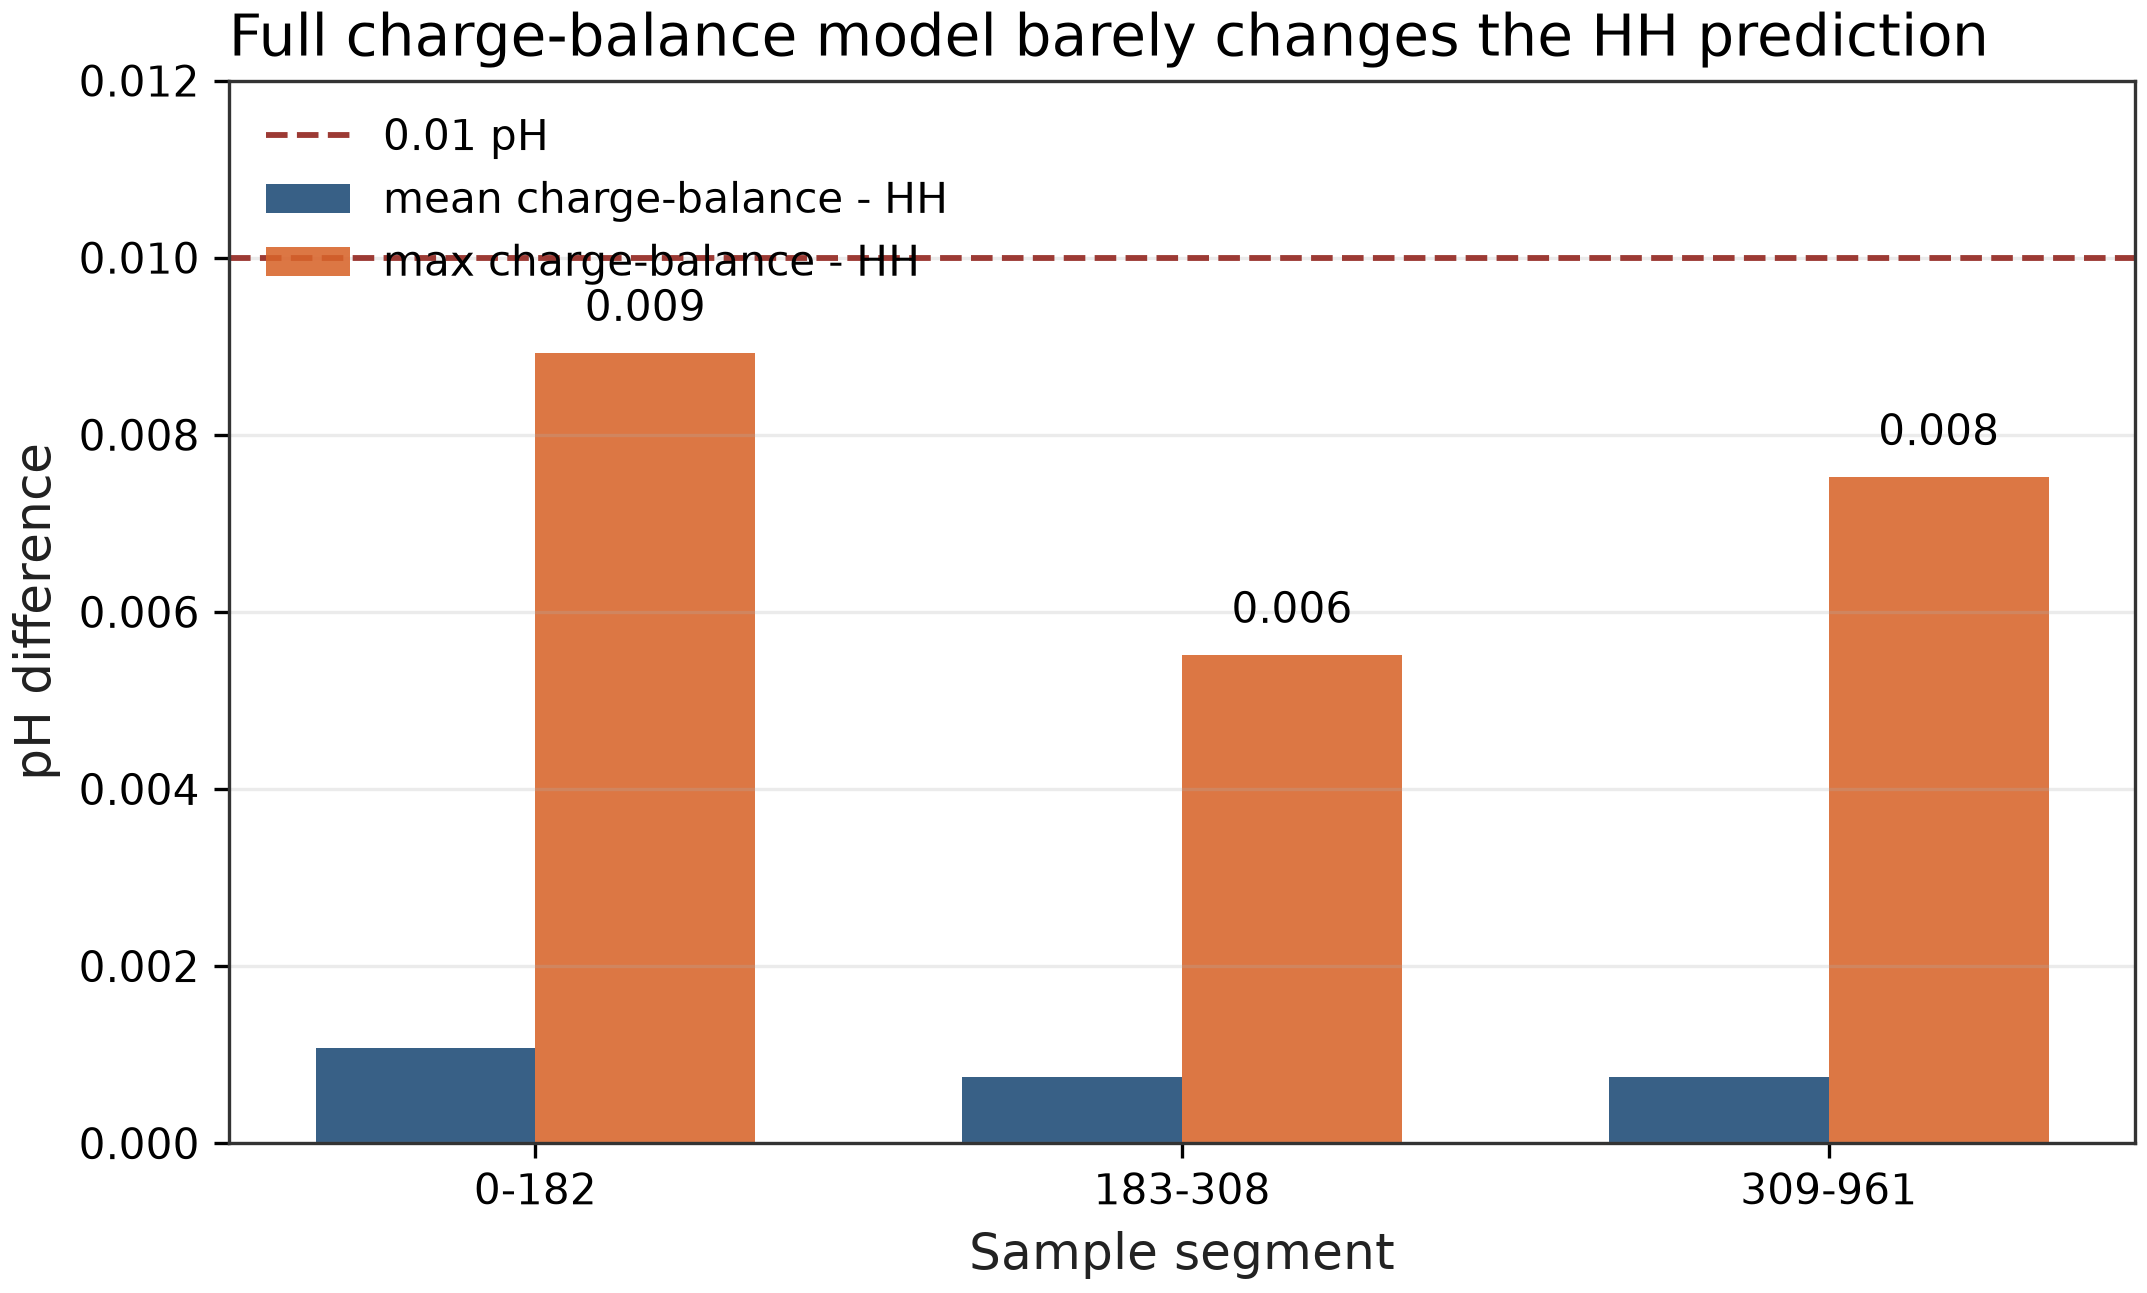
\includegraphics[width=\linewidth,height=0.74\textheight,keepaspectratio]{slide_water_charge_balance.png}
\end{column}
\end{columns}
\end{frame}

%============================= Slide 2 ============================
\begin{frame}
\setbeamertemplate{blocks}[rounded][shadow=false]
\setbeamercolor{block body}{fg=black,bg=blockTint}
\frametitle{\large \textbf{Updated dataset: sequential view of flows and PH\_2}}
\scriptsize

\vspace{-0.22cm}
\centering
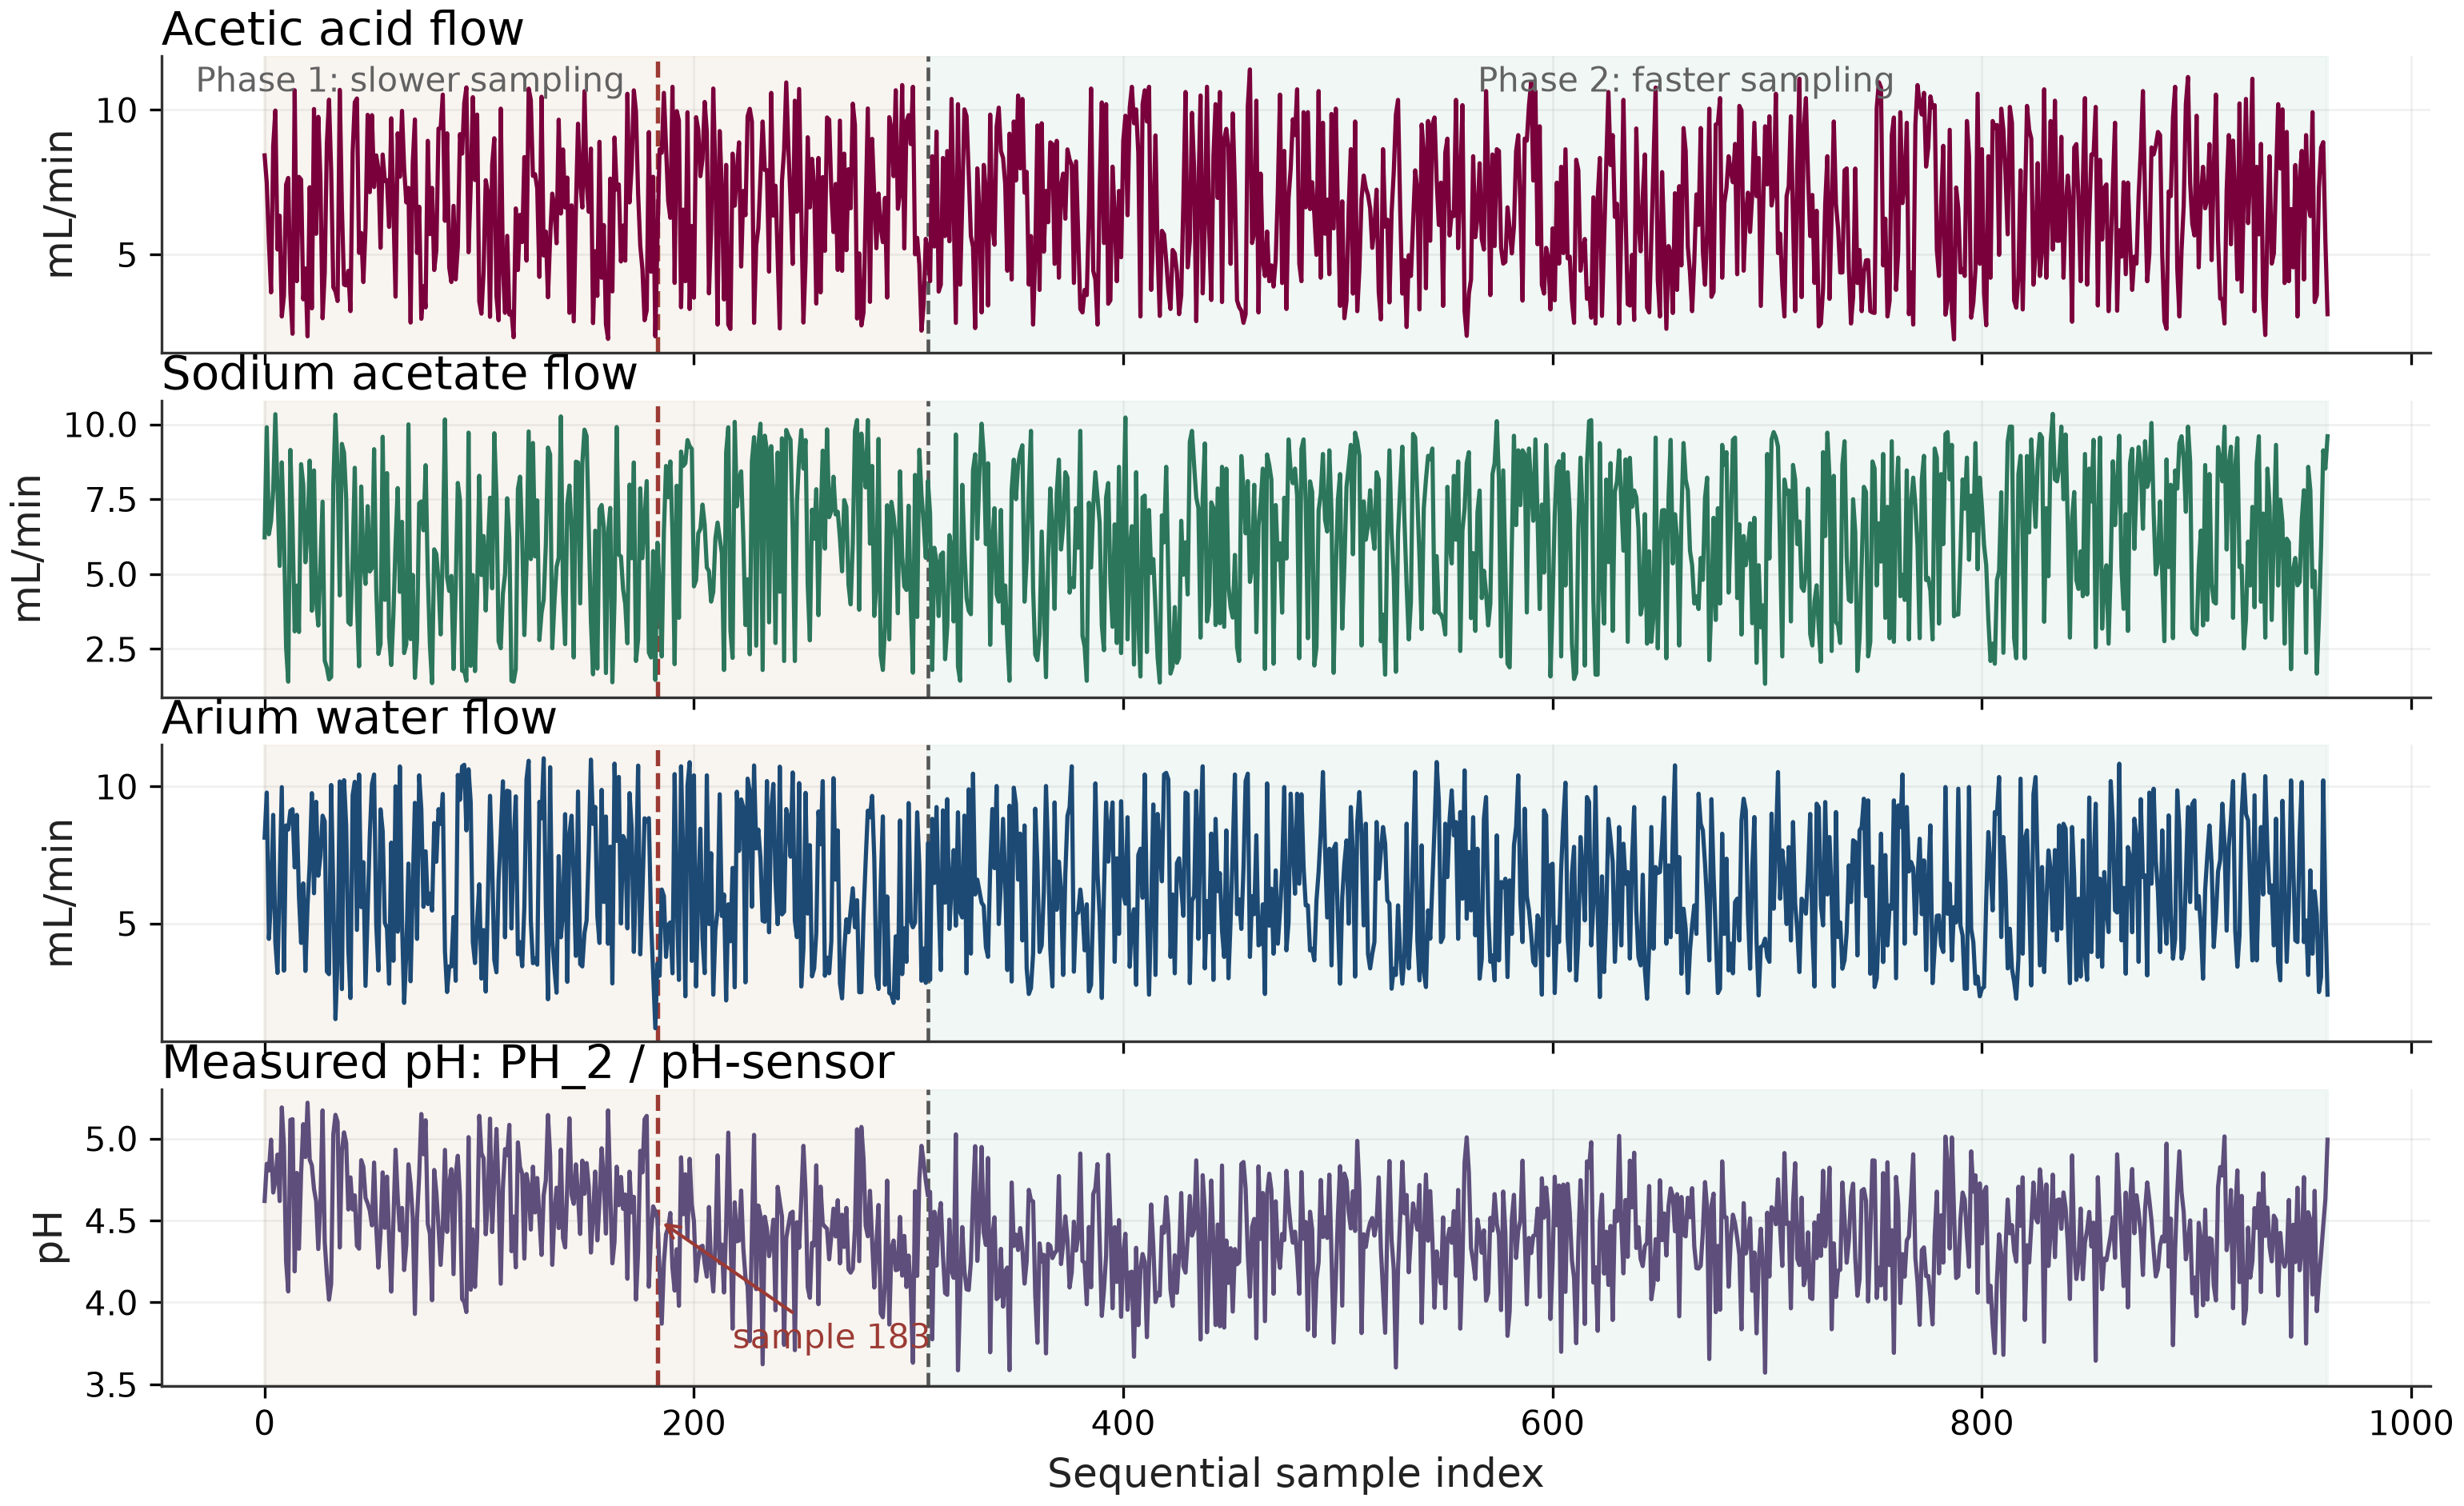
\includegraphics[width=0.98\linewidth,height=0.78\textheight,keepaspectratio]{slide_data_overview.png}

\vspace{-0.05cm}
\begin{beamercolorbox}[rounded=true,center,sep=3.5pt,wd=0.95\linewidth]{block body}
{\bfseries Small interpretation:} x-axis is sample index. Sample 183 is the main residual-shift boundary; sample 309 is only the sampling-rate phase change.
\end{beamercolorbox}
\end{frame}

%============================= Slide 3 ============================
\begin{frame}
\setbeamertemplate{blocks}[rounded][shadow=false]
\setbeamercolor{block body}{fg=black,bg=blockTint}
\frametitle{\large \textbf{HH prediction tracks the trend, but the residual becomes biased}}
\scriptsize

\vspace{-0.20cm}
\centering
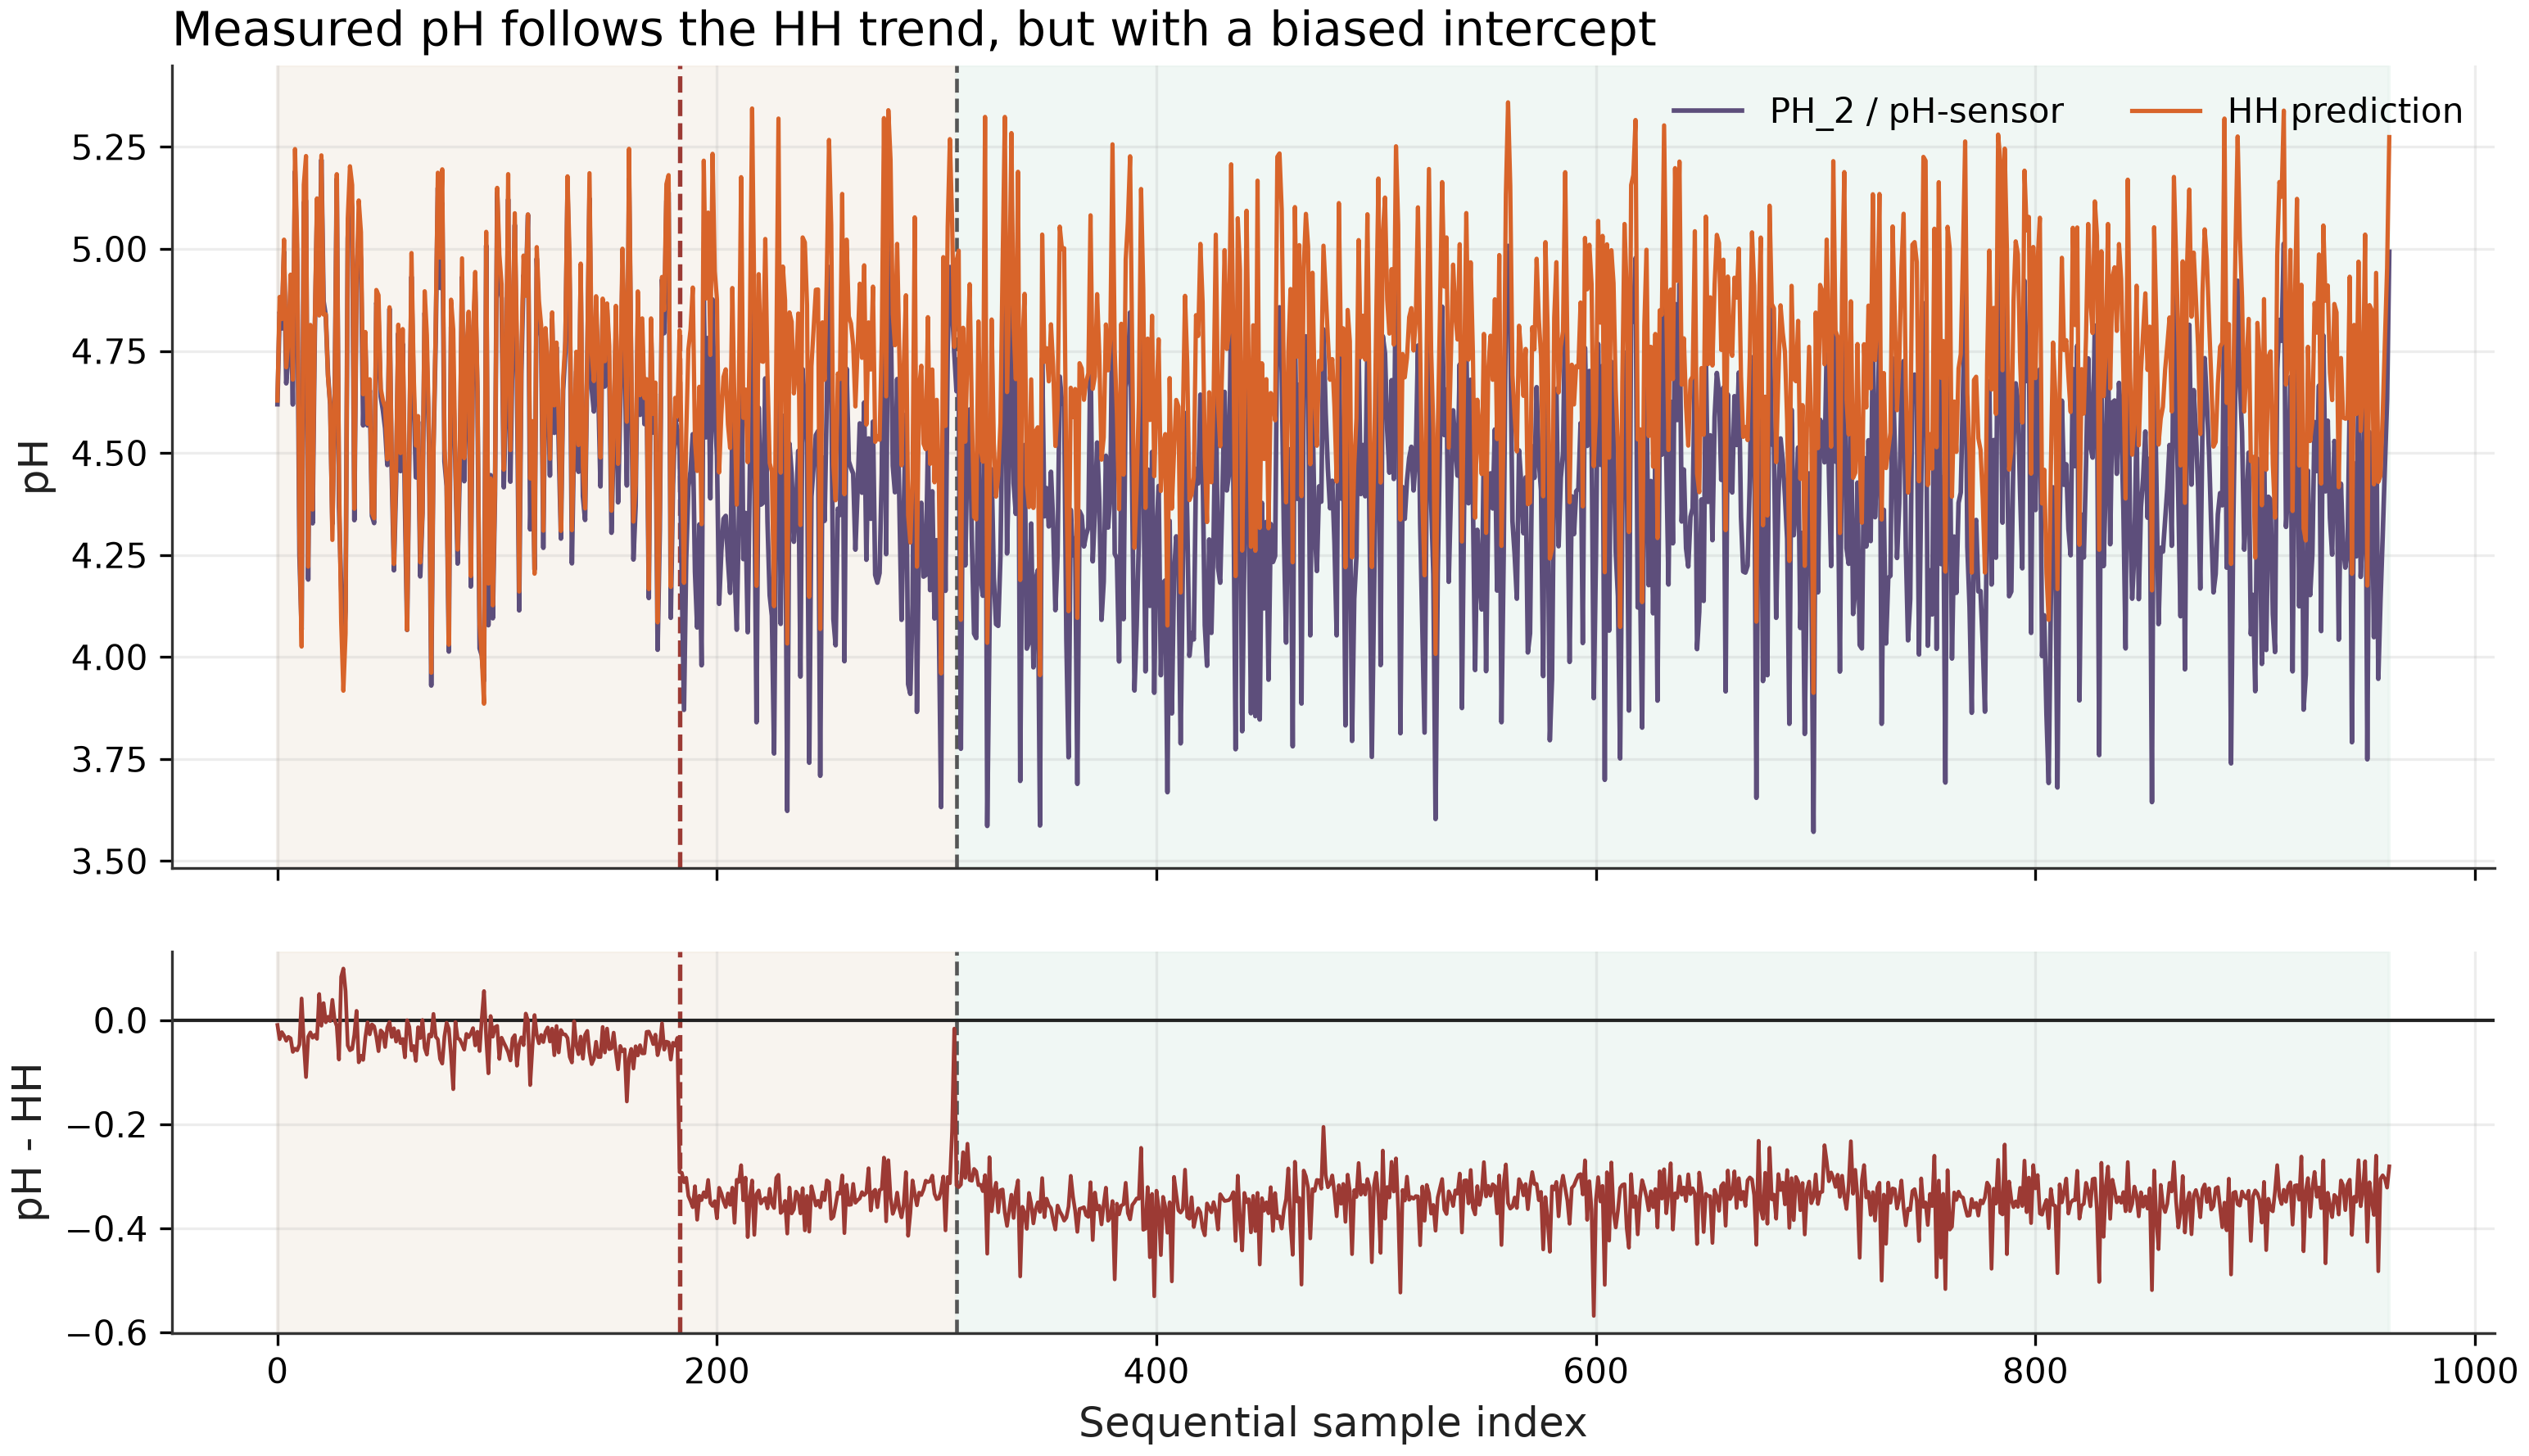
\includegraphics[width=0.98\linewidth,height=0.74\textheight,keepaspectratio]{slide_hh_prediction_residual.png}

\vspace{-0.03cm}
\begin{columns}[T,onlytextwidth]
\begin{column}{0.58\textwidth}
\begin{beamercolorbox}[rounded=true,center,sep=3.5pt,wd=\linewidth]{block body}
Overall: mean error $=-0.286$, MAE $=0.287$, RMSE $=0.314$, correlation $=0.913$.
\end{beamercolorbox}
\end{column}
\begin{column}{0.39\textwidth}
\begin{beamercolorbox}[rounded=true,center,sep=3.5pt,wd=\linewidth]{block body}
Bias is an intercept problem more than a ratio-trend problem.
\end{beamercolorbox}
\end{column}
\end{columns}
\end{frame}

%============================= Slide 4 ============================
\begin{frame}
\setbeamertemplate{blocks}[rounded][shadow=false]
\setbeamercolor{block body}{fg=black,bg=blockTint}
\frametitle{\large \textbf{The residual shift occurs at the overnight/session boundary}}
\scriptsize

\vspace{-0.20cm}
\centering
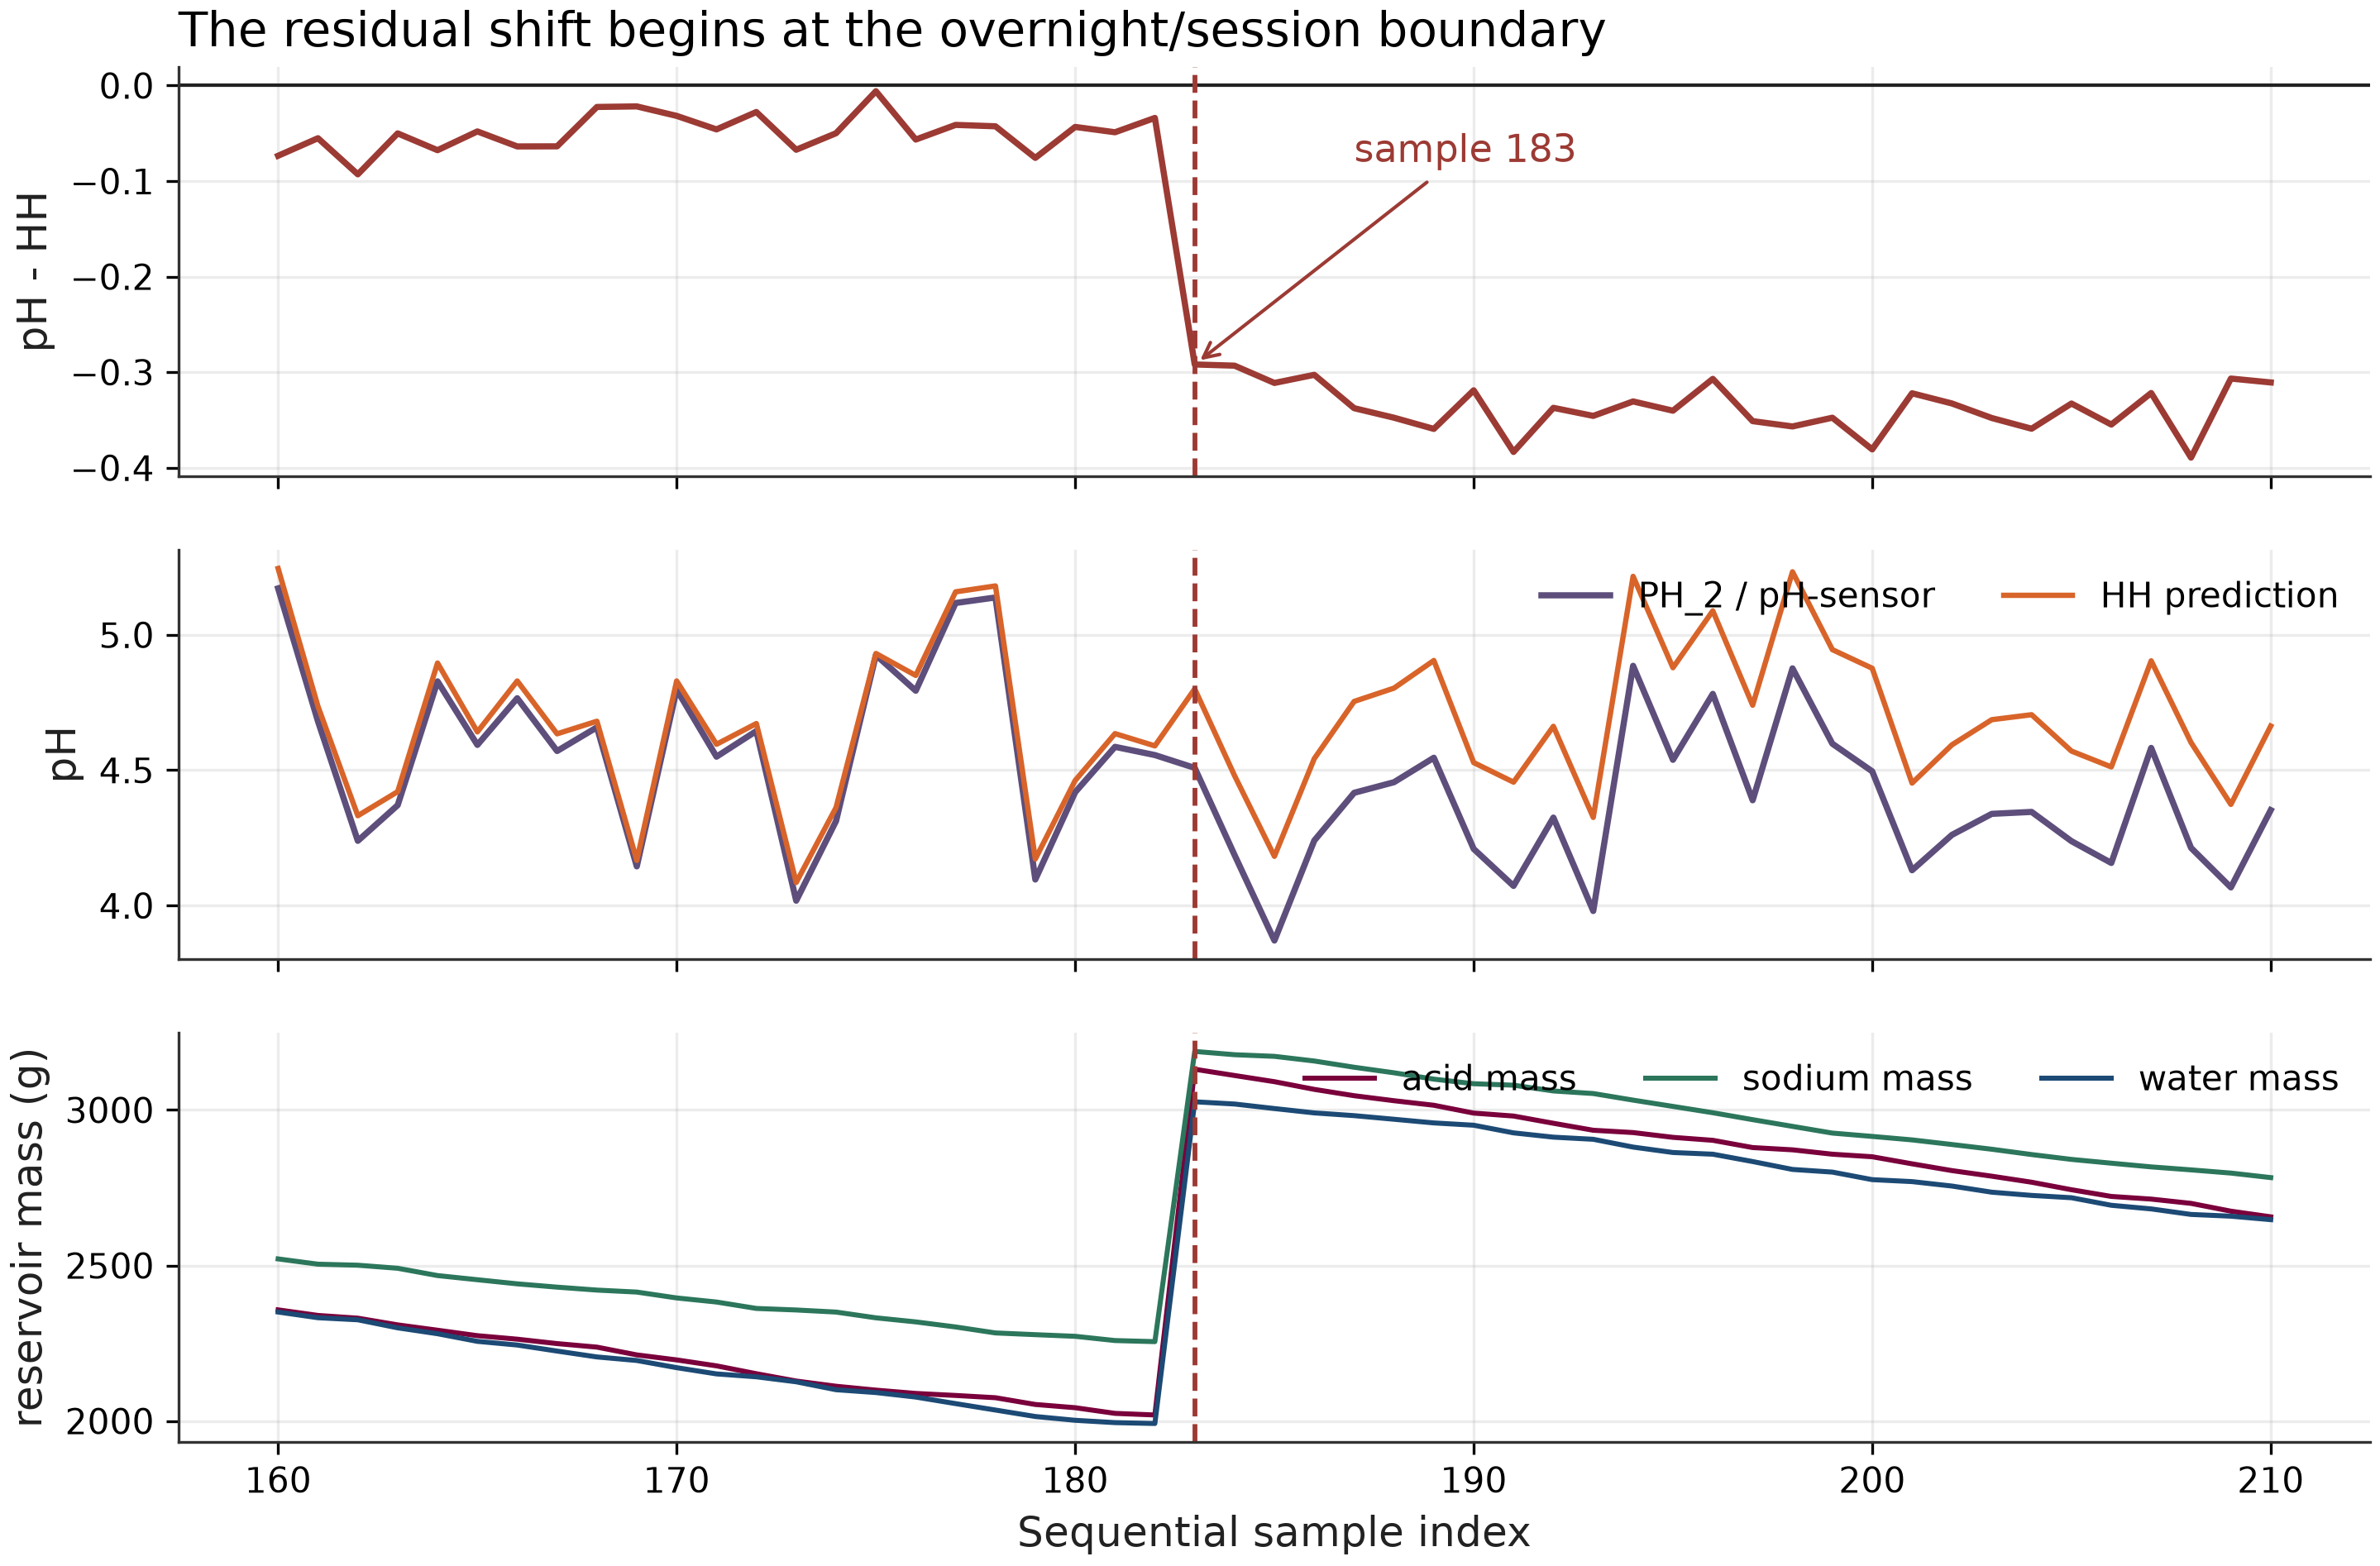
\includegraphics[width=0.98\linewidth,height=0.77\textheight,keepaspectratio]{slide_shift_context.png}

\vspace{-0.04cm}
\begin{beamercolorbox}[rounded=true,center,sep=3.5pt,wd=0.95\linewidth]{block body}
{\bfseries Small interpretation:} after sample 183, PH\_2 remains below the HH prediction while reservoir masses reset upward.
\end{beamercolorbox}
\end{frame}

%============================= Slide 5 ============================
\begin{frame}
\setbeamertemplate{blocks}[rounded][shadow=false]
\setbeamercolor{block body}{fg=black,bg=blockTint}
\frametitle{\large \textbf{Apparent pKa confirms a regime-dependent intercept shift}}
\scriptsize

\vspace{-0.20cm}
\centering
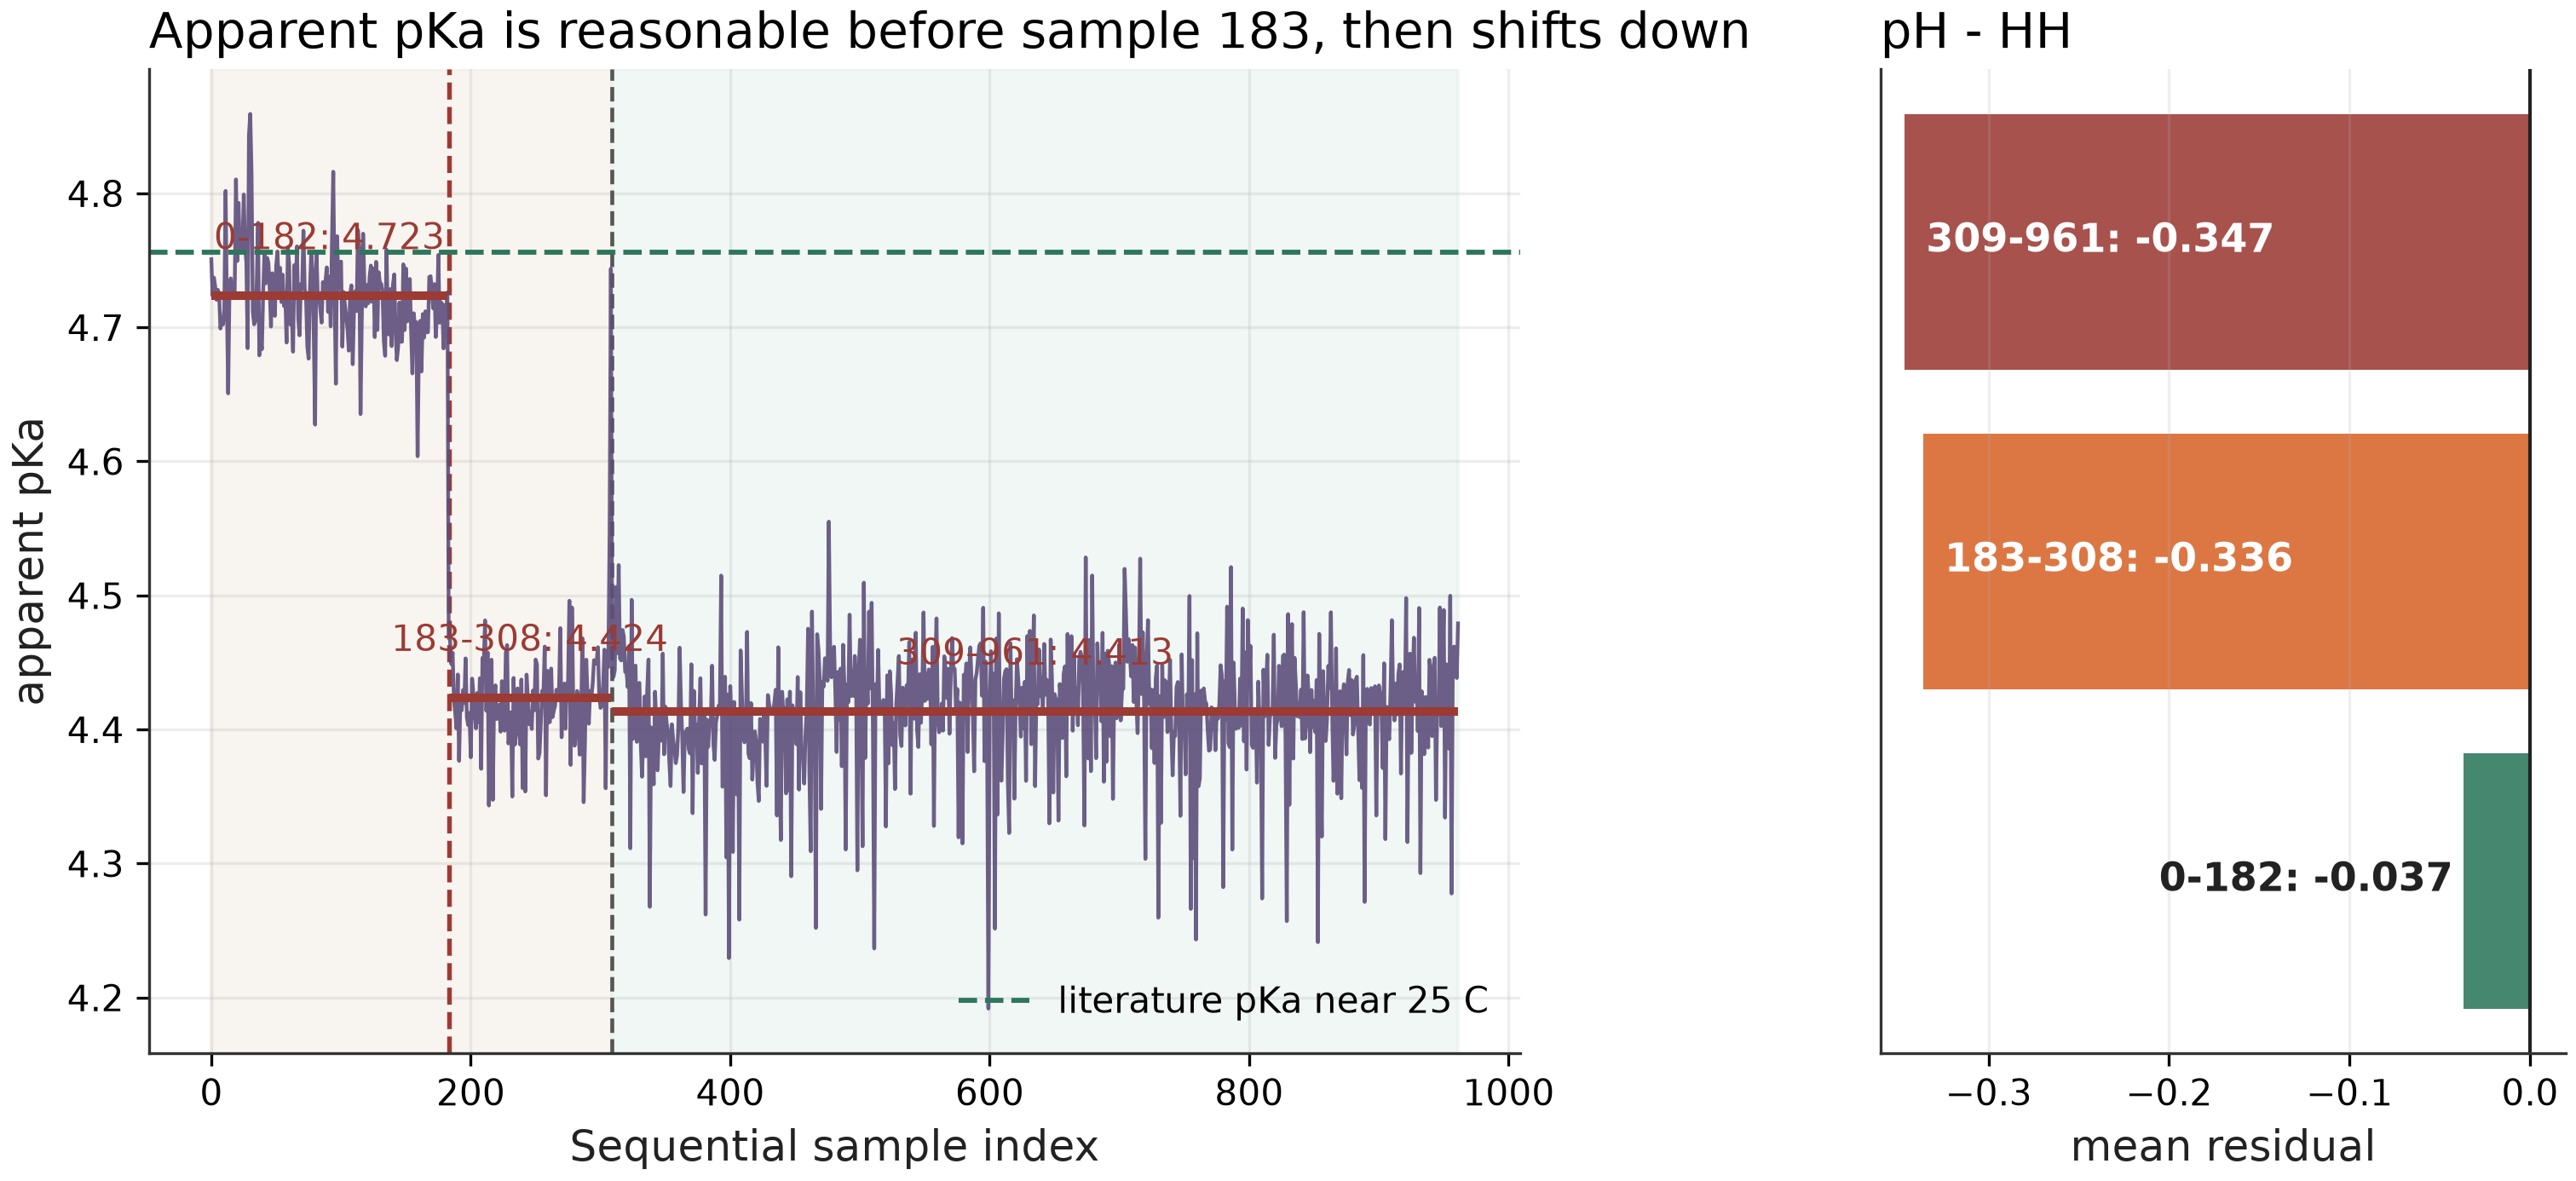
\includegraphics[width=0.98\linewidth,height=0.73\textheight,keepaspectratio]{slide_pka_regime_summary.png}

\vspace{-0.02cm}
\begin{columns}[T,onlytextwidth]
\begin{column}{0.50\textwidth}
\begin{beamercolorbox}[rounded=true,center,sep=3.5pt,wd=\linewidth]{block body}
$pK_{a,\mathrm{app},k}=\pH_k-\log_{10}(F_{acetate,k}/F_{acid,k})$
\end{beamercolorbox}
\end{column}
\begin{column}{0.47\textwidth}
\begin{beamercolorbox}[rounded=true,center,sep=3.5pt,wd=\linewidth]{block body}
Post-183 value is not a normal temperature pKa.
\end{beamercolorbox}
\end{column}
\end{columns}
\end{frame}

%============================= Slide 6 ============================
\begin{frame}
\setbeamertemplate{blocks}[rounded][shadow=false]
\setbeamercolor{block body}{fg=black,bg=blockTint}
\frametitle{\large \textbf{Raw three-flow control is non-unique for pH tracking}}
\scriptsize

\vspace{-0.12cm}
\begin{columns}[T,onlytextwidth]
\begin{column}{0.40\textwidth}
\begin{block}{Problem with raw actions}
\vspace{-0.12cm}
\[
  u=\begin{bmatrix}F_{acid}\\F_{acetate}\\F_W\end{bmatrix},
  \qquad
  \pH\approx pK_a+\log_{10}\frac{F_{acetate}}{F_{acid}}
\]
\vspace{-0.20cm}
\[
  (1,1),\ (3,3),\ (8,8)
  \quad\Rightarrow\quad
  F_{acetate}/F_{acid}=1
\]
\vspace{-0.15cm}
\end{block}

\vspace{0.04cm}
\begin{block}{Document warning}
\begin{itemize}\raggedright
  \setlength\itemsep{0.35ex}
  \item drifting to unnecessarily high flows,
  \item drifting to very low flows,
  \item unstable/chattering pump actions,
  \item meaningless use of water or total flow.
\end{itemize}
\end{block}
\end{column}

\begin{column}{0.58\textwidth}
\centering
\resizebox{0.96\linewidth}{!}{%
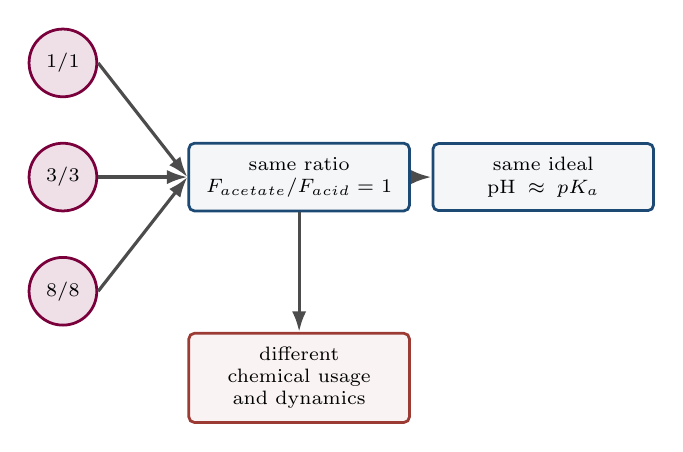
\begin{tikzpicture}[
  point/.style={circle,draw=maroon1,fill=maroon1!12,line width=1.0pt,minimum size=0.86cm,font=\scriptsize,align=center},
  arr/.style={-{Latex[length=2.6mm,width=1.8mm]},line width=1.15pt,draw=black!70},
  box/.style={draw=maccblue,line width=1.0pt,rounded corners=2pt,align=center,fill=maccblue!5,
    text width=2.45cm,inner sep=5pt,font=\scriptsize}
]
\node[point] (a) at (0,1.45) {$1/1$};
\node[point] (b) at (0,0.00) {$3/3$};
\node[point] (c) at (0,-1.45) {$8/8$};
\node[box] (ratio) at (3.0,0) {same ratio\\$F_{acetate}/F_{acid}=1$};
\node[box] (ph) at (6.1,0) {same ideal\\$\pH\approx pK_a$};
\node[box,draw=maccred,fill=maccred!6] (usage) at (3.0,-2.55) {different\\chemical usage\\and dynamics};
\draw[arr] (a.east) -- (ratio.west);
\draw[arr] (b.east) -- (ratio.west);
\draw[arr] (c.east) -- (ratio.west);
\draw[arr] (ratio.east) -- (ph.west);
\draw[arr] (ratio.south) -- (usage.north);
\end{tikzpicture}}

\vspace{0.22cm}
\begin{beamercolorbox}[rounded=true,center,sep=4pt,wd=0.92\linewidth]{block body}
The pH reward alone cannot choose the ``best'' flow pair.
\end{beamercolorbox}
\end{column}
\end{columns}
\end{frame}

%============================= Slide 7 ============================
\begin{frame}
\setbeamertemplate{blocks}[rounded][shadow=false]
\setbeamercolor{block body}{fg=black,bg=blockTint}
\frametitle{\large \textbf{Controller structure 1: ratio-based controller}}
\scriptsize

\vspace{-0.12cm}
\begin{columns}[T,onlytextwidth]
\begin{column}{0.40\textwidth}
\begin{block}{Reparameterize the action}
\vspace{-0.12cm}
\[
  r=\frac{F_{acetate}}{F_{acid}},
  \qquad
  z=\log_{10}\frac{F_{acetate}}{F_{acid}}
\]
\vspace{-0.18cm}
\[
  \pH \approx pK_a+z,
  \qquad
  F_B=F_{acid}+F_{acetate}
\]
\vspace{-0.16cm}
\end{block}

\vspace{0.04cm}
\begin{block}{Deterministic flow allocator}
\vspace{-0.12cm}
\[
  r=10^z,\quad
  F_{acid}=\frac{F_B}{1+r},\quad
  F_{acetate}=\frac{rF_B}{1+r}
\]
\vspace{-0.16cm}
\end{block}
\end{column}

\begin{column}{0.58\textwidth}
\centering
\resizebox{1.00\linewidth}{!}{%
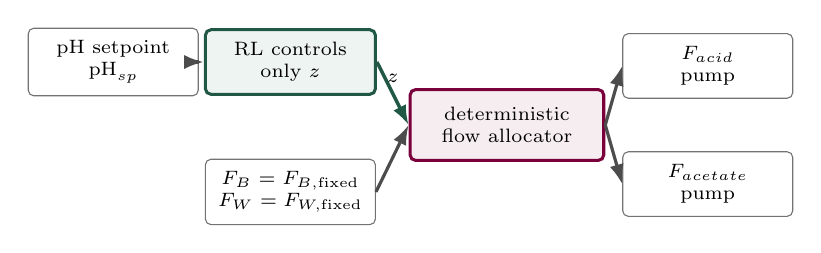
\begin{tikzpicture}[
  box/.style={draw=black!55,rounded corners=2pt,align=center,fill=white,
    inner sep=4.4pt,text width=1.85cm,minimum height=0.82cm,font=\scriptsize},
  cmd/.style={draw=maccgreen!75!black,line width=1.1pt,rounded corners=2pt,align=center,fill=maccgreen!8,
    inner sep=4.4pt,text width=1.85cm,minimum height=0.82cm,font=\scriptsize},
  alloc/.style={draw=maroon1,line width=1.1pt,rounded corners=2pt,align=center,fill=maroon1!7,
    inner sep=4.4pt,text width=2.15cm,minimum height=0.90cm,font=\scriptsize},
  arr/.style={-{Latex[length=2.5mm,width=1.8mm]},line width=1.15pt,draw=black!70},
  garr/.style={-{Latex[length=2.5mm,width=1.8mm]},line width=1.25pt,draw=maccgreen!75!black}
]
\node[box] (sp) at (0.0,1.2) {pH setpoint\\$\pH_{sp}$};
\node[cmd] (rl) at (2.25,1.2) {RL controls\\only $z$};
\node[box] (fb) at (2.25,-0.45) {$F_B=F_{B,\mathrm{fixed}}$\\$\FW=F_{W,\mathrm{fixed}}$};
\node[alloc] (alloc) at (5.00,0.40) {deterministic\\flow allocator};
\node[box] (acid) at (7.55,1.15) {$F_{acid}$\\pump};
\node[box] (base) at (7.55,-0.35) {$F_{acetate}$\\pump};
\draw[arr] (sp.east) -- (rl.west);
\draw[garr] (rl.east) -- node[above,font=\scriptsize] {$z$} (alloc.west);
\draw[arr] (fb.east) -- (alloc.west);
\draw[arr] (alloc.east) -- (acid.west);
\draw[arr] (alloc.east) -- (base.west);
\end{tikzpicture}}

\vspace{0.20cm}
\begin{beamercolorbox}[rounded=true,center,sep=4pt,wd=0.92\linewidth]{block body}
First RL version: RL controls only $z$; $F_B$ and $\FW$ are fixed or chosen by a simple rule.
\end{beamercolorbox}
\end{column}
\end{columns}
\end{frame}

%============================= Slide 8 ============================
\begin{frame}
\setbeamertemplate{blocks}[rounded][shadow=false]
\setbeamercolor{block body}{fg=black,bg=blockTint}
\frametitle{\large \textbf{Controller structures 2--3: correction and usage objective}}
\scriptsize

\vspace{-0.14cm}
\begin{columns}[T,onlytextwidth]
\begin{column}{0.48\textwidth}
\begin{block}{HH baseline + RL correction}
\vspace{-0.12cm}
\[
  z_{HH}=\pH_{sp}-pK_a,
  \qquad
  z_{RL}=z_{HH}+\Delta z_{RL}
\]
\vspace{-0.18cm}
\[
  r=10^{z_{RL}},
  \qquad
  F_{acid}=\frac{F_B}{1+r},
  \qquad
  F_{acetate}=\frac{rF_B}{1+r}
\]
\vspace{-0.15cm}
\end{block}

\vspace{0.04cm}
\begin{block}{$\Delta z_{RL}$ corrects}
\begin{itemize}\raggedright
  \setlength\itemsep{0.35ex}
  \item sensor bias,
  \item mixing delay,
  \item activity effects,
  \item model mismatch.
\end{itemize}
\end{block}
\end{column}

\begin{column}{0.49\textwidth}
\begin{block}{Chemical usage objective}
\vspace{-0.12cm}
\[
  \begin{aligned}
  R_k =&
  -Q(\pH_k-\pH_{sp})^2
  -\lambda_{\Delta u}\|\Delta u_k\|^2\\
  &-\lambda_B(F_B-F_{B,ref})^2
  -\lambda_{chem}(F_{acid}+F_{acetate})
  \end{aligned}
\]
\vspace{-0.18cm}
\[
  C_{buffer}\ge C_{min}
  \qquad
  C_{buffer}=
  \frac{C_0(F_{acid}+F_{acetate})}{F_{acid}+F_{acetate}+\FW}
\]
\vspace{-0.16cm}
\end{block}

\vspace{0.04cm}
\begin{block}{Clean hierarchy from the document}
\begin{tabular}{@{}ll@{}}
pH tracking & control acid/acetate ratio\\
buffer strength & control total acid+acetate flow\\
dilution/residence time & control water or total flow\\
\end{tabular}
\end{block}
\end{column}
\end{columns}
\end{frame}

\end{document}
